\documentclass[11pt]{article}
\usepackage[a4paper,margin=1in]{geometry}
\usepackage{enumitem}
\usepackage{hyperref}
\usepackage{amsmath}
\usepackage{pgfplots}

\pgfplotsset{compat=1.18}

\title{Mental Math Progression \& Level System (v1)}
\date{}

\begin{document}

\maketitle

\section{Vision}

\begin{itemize}[leftmargin=*]
    \item No global Elo system.
    \item Personalized progression per user.
    \item Each level corresponds to a \textbf{pattern family}.
    \item Progression based on:
    \begin{itemize}
        \item Relative speed (time-to-first-correct; median vs population)
        \item Skip behavior
    \end{itemize}
    \item Long-term target: remove hard-coded thresholds and use population-adaptive percentiles.
\end{itemize}

In v1, cutoffs are hard-coded for simplicity; later versions can fully adapt automatically using population response-time percentiles.

\section{High-Level Structure}

Progression is separated by \textbf{Operation Domains}:

\begin{itemize}[leftmargin=*]
    \item Addition (ADD)
    \item Multiplication (MUL)
    \item Subtraction (SUB)
    \item Division (DIV)
\end{itemize}

Each domain has its own independent level ladder.

User progress is tracked per domain.

\section{Pattern-Based Levels}

Each level corresponds to a defined structural pattern.

A pattern is \textbf{not} a single question. It is a generator rule with structural constraints.

Each pattern contains:

\begin{itemize}[leftmargin=*]
    \item Operation
    \item Digit configuration
    \item Carry constraints (operation-specific)
    \item Other structural constraints (pattern-specific)
\end{itemize}

\subsection*{Operand Order Randomization}

For all patterns involving operands of different digit lengths, 
the order of the operands is randomized at generation time 
(e.g., $1$-digit $+$ $2$-digit or $2$-digit $+$ $1$-digit).
For equal-length operands (e.g., $1$-digit $+$ $1$-digit), 
order is naturally symmetric.

\subsection*{Example Patterns (Addition) --- first 5 levels}

\begin{itemize}[leftmargin=*]
    \item Level 1: 1-digit + 1-digit, no carry
    \item Level 2: 1-digit + 1-digit, with carry
    \item Level 3: 1-digit + 2-digit, no carry
    \item Level 4: 1-digit + 2-digit, with carry
    \item Level 5: 2-digit + 2-digit, no carry
\end{itemize}

\subsection*{Example Patterns (Multiplication) --- first 5 levels}

\begin{itemize}[leftmargin=*]
    \item Level 1: 1-digit $\times$ 1-digit, no carry
    \item Level 2: 1-digit $\times$ 1-digit, with carry
    \item Level 3: 1-digit $\times$ 2-digit, no carry
    \item Level 4: 1-digit $\times$ 2-digit, with carry
    \item Level 5: 1-digit $\times$ 2-digit, two carries
\end{itemize}

\subsection*{Example Patterns (Subtraction) --- first 5 levels}

\begin{itemize}[leftmargin=*]
    \item Level 1: 1-digit $-$ 1-digit, non-negative result (no borrow possible)
    \item Level 2: 2-digit $-$ 1-digit, no borrow
    \item Level 3: 2-digit $-$ 1-digit, with borrow (single borrow)
    \item Level 4: 2-digit $-$ 2-digit, no borrow
    \item Level 5: 2-digit $-$ 2-digit, with borrow (single borrow)
\end{itemize}


\subsection*{Example Patterns (Division) --- first 5 levels }

\begin{itemize}[leftmargin=*]
    \item Level 1: 1-digit $\div$ 1-digit, exact integer result
    \item Level 2: 2-digit $\div$ 1-digit, exact integer result
    \item Level 3: 2-digit $\div$ 2-digit, exact integer result
    \item Level 4: 3-digit $\div$ 1-digit, exact integer result
    \item Level 5: 3-digit $\div$ 2-digit, exact integer result
\end{itemize}



\section{Performance Model (v1: Hard-Coded Cutoff)}

Progression is based on:

\begin{itemize}[leftmargin=*]
    \item Whether the attempt is solved (correct answer submitted within $C_L$ milliseconds)
    \item If time-to-first-correct exceeds $C_L$, the attempt counts as unsolved regardless of correctness
\end{itemize}

For v1, each (domain, level) has a hard-coded \textbf{cutoff time} $C_L$.

This threshold is tuned manually and can later be replaced by population percentiles.

\section{Promotion Rule (Per Level)}

For a user currently on Level $L$ in a domain, evaluate the last $N$ completed attempts at Level $L$.

\begin{center}
$N = 10$
\end{center}

Promotion requires:

\begin{enumerate}[leftmargin=*]
    \item All of the last $N$ attempts are solved (correct and within $C_L$)
\end{enumerate}

If satisfied, unlock Level $L + 1$.

\section{Demotion Rule (Hysteresis)}

Evaluate the last $M$ attempts at the current level (including skips).

\begin{center}
$M = 20$
\end{center}

Demote if any of the following holds:

\begin{itemize}[leftmargin=*]
    \item Unsolved rate over the last $M$ attempts exceeds tolerance $S_{max}$
\end{itemize}

\begin{itemize}[leftmargin=*]
    \item $S_{max} = 0.25$ (25\%)
\end{itemize}

Only allow demotion after a minimum exposure at that level (20 attempts).

\subsection*{Soft Demotion Target}

Demotion is intentionally soft:

\begin{itemize}[leftmargin=*]
    \item If the user is at level $L$, a demotion moves to $L-1$ (minimum level is $1$).
    \item This is true even if the triggering failures happened on a sampled lower level $k < L$.
    \item Example: if user is at level $10$ and repeated failures are observed on level $8$ questions, demotion target is level $9$ (not level $7$).
\end{itemize}

Formally:

\[
L_{new} = \max(1, L - 1)
\]

\section{Level Selection During Play}

Let the user's current level in a domain be $L$. During play, sample question level $k$ from the set:

\[
k \in \{1,2,\dots,L,L+1\}
\]

Use fixed top-level buckets:

\[
p(L)=0.50, \qquad p(L+1)=0.10
\]

The remaining mass is assigned to all lower levels:

\[
\sum_{k=1}^{L-1} p(k)=0.40
\]

Distribute this $0.40$ over levels $1..L-1$ with geometric taper:

\[
u(k)=r^{(L-1)-k}, \qquad 1 \le k \le L-1, \quad 0<r<1
\]

\[
p(k)=0.40\cdot\frac{u(k)}{\sum_{j=1}^{L-1} u(j)}, \qquad 1 \le k \le L-1
\]

\[
\text{If } L=1:\quad p(1)=0.90,\; p(2)=0.10
\]

So the current level is always most likely, the next level is fixed at $10\%$, and all lower levels remain possible with decreasing probability.

\subsection*{Symbol definitions}

\begin{itemize}[leftmargin=*]
    \item $L$: current user level in the domain
    \item $k$: sampled question level
    \item $r \in (0,1)$: geometric decay factor for lower levels (smaller $r$ means faster taper)
    \item $u(k)$: unnormalized geometric weight for lower levels
\end{itemize}

\subsection*{Stability after demotion}

The level sampling rule above is always the same, regardless of why a demotion happened.
After demotion, only $L$ changes; the same weighting formula and hyperparameters are reused.

\subsection*{Example distribution (bar chart)}

Example with $L=10$ and $r=0.6$ (final $p(k)$):

\begin{center}
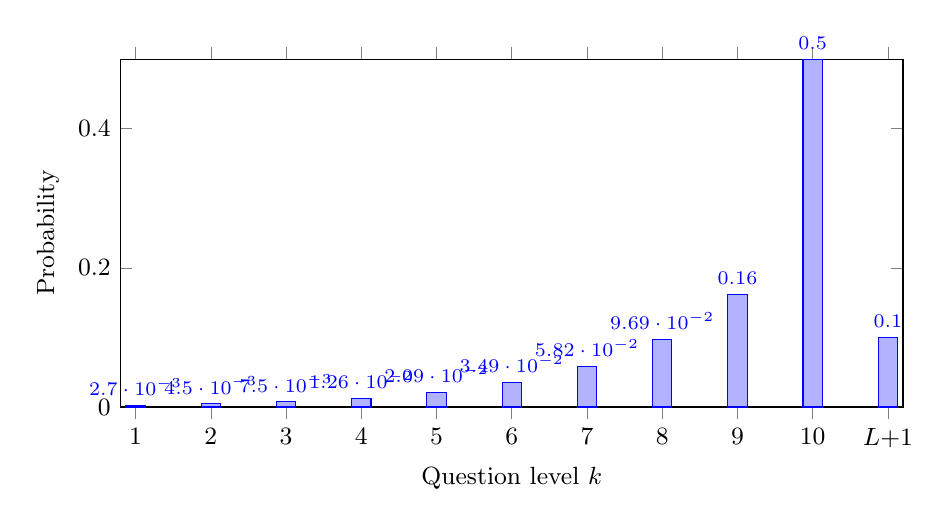
\begin{tikzpicture}
\begin{axis}[
    ybar,
    width=0.95\linewidth,
    height=6.0cm,
    ymin=0,
    ymax=0.5,
    ylabel={Probability},
    xlabel={Question level $k$},
    xtick={1,2,3,4,5,6,7,8,9,10,11},
    xticklabels={1,2,3,4,5,6,7,8,9,10,$L{+}1$},
    bar width=7pt,
    enlarge x limits=0.02,
    nodes near coords,
    nodes near coords align={vertical},
    every node near coord/.append style={font=\scriptsize},
    tick label style={font=\small},
    label style={font=\small}
]
\addplot coordinates {
    (1,0.0027)
    (2,0.0045)
    (3,0.0075)
    (4,0.0126)
    (5,0.0209)
    (6,0.0349)
    (7,0.0582)
    (8,0.0969)
    (9,0.1616)
    (10,0.5000)
    (11,0.1000)
};
\end{axis}
\end{tikzpicture}
\end{center}

Within a level:

\begin{itemize}[leftmargin=*]
    \item Randomize seeds
    \item Randomize digit combinations
    \item Maintain structural constraints
\end{itemize}



\section{How Questions are stored}

\begin{enumerate}[leftmargin=*]
    \item Store \textbf{Pattern} rows (the generator rules).
    \item Generate question instances on demand using a RNG seed.
    \item Store each user interaction as an \textbf{Attempt} row.
\end{enumerate}

So, in practice, the ``question'' is represented by:

\begin{center}
\texttt{(patternId, seed)}
\end{center}

Optional later: add a \texttt{QuestionInstance} table only if you need explicit review queues or caching.

\subsection*{How a Pattern is stored in DB}

Each pattern family is one row in the \texttt{pattern} table.

Stable, indexed fields are stored as normal columns:

\begin{itemize}[leftmargin=*]
        \item \texttt{id}: unique pattern id
        \item \texttt{domain}: \texttt{ADD | MUL | SUB | DIV}
        \item \texttt{level}: ladder level within domain
        \item \texttt{description}: human-readable pattern label
        \item \texttt{cutoffTimeMs}: solved-time cutoff for v1
        \item \texttt{active}: enable/disable pattern
        \item \texttt{createdAt}, \texttt{updatedAt}: audit timestamps
\end{itemize}

Dynamic generation constraints are stored in:

\begin{itemize}[leftmargin=*]
        \item \texttt{params} (Prisma \texttt{Json}, PostgreSQL \texttt{JSONB})
\end{itemize}

Uniqueness rule in v1:

\begin{center}
\texttt{UNIQUE(domain, level, description)}
\end{center}

\subsection*{What \texttt{params} JSON looks like}

In v1, digit fields are stored as single integers (not lists),
because each pattern uses one fixed digit size per side.

\textbf{ADD example (Level 3: 1-digit + 2-digit, no carry)}

\begin{verbatim}
{
    "operation": "ADD",
    "leftDigits": 1,
    "rightDigits": 2,
    "carryCount": 0,
}
\end{verbatim}

\textbf{MUL example (Level 5: 1-digit x 2-digit, two carries)}

\begin{verbatim}
{
    "operation": "MUL",
    "leftDigits": 1,
    "rightDigits": 2,
    "carryCount": 2,
}
\end{verbatim}

\textbf{SUB example (Level 5: 2-digit - 2-digit, single borrow)}

\begin{verbatim}
{
    "operation": "SUB",
    "leftDigits": 2,
    "rightDigits": 2,
    "borrowCount": 1,
    "allowNegative": false
}
\end{verbatim}

\textbf{DIV example (Level 3: 2-digit / 2-digit, exact integer)}

\begin{verbatim}
{
    "operation": "DIV",
    "dividendDigits": 2,
    "divisorDigits": 2,
    "exactInteger": true,
    "minQuotient": 2
}
\end{verbatim}

The exact key set may vary by operation and version. The important rule is:
keep frequently queried fields in columns and operation-specific constraints in \texttt{params}.

\end{document}
